% +------------------------------------------------------------------------+
% | Reference manual page: SubdivisionMask_3.tex
% +------------------------------------------------------------------------+
% | 03.17.2006 Andy Shiue
% | Package: Subdivision_method_3
% | 
\RCSdef{\RCSSubdivisionMaskRev}{$Id$}
\RCSdefDate{\RCSSubdivisionMaskDate}{$Date$}




% +------------------------------------------------------------------------+
\ccRefPageBegin
% +------------------------------------------------------------------------+

\begin{ccRefConcept}{PQQMask_3}
\label{pagePQQMaskRef}  

Required member functions for the \ccRefName\ concept. This
policy concept of geometric computations is used in
\ccc{CGAL::Subdivision_method_3::PQQ<Polyhedron_3, Mask>}.


%\ccTypes

%\ccNestedType{Point_3}{point type.}

\ccCreationVariable{mask}

\ccOperations
\ccSetThreeColumns{facet_node}{}{\hspace*{8.5cm}}

\ccMethod{void facet_node(Facet_handle facet, Point_3& pt);}{
    computes the facet-point \ccc{pt} based on the neighborhood
    of the facet \ccc{f}.}

\ccMethod{void edge_node(Edge_handle e, Point_3& pt);}{
    computes the edge-point \ccc{pt} based on the neighborhood
    of the edge \ccc{e}.}

\ccMethod{void vertex_node(Vertex_handle v, Point_3& pt);}{
    computes the vertex-point \ccc{pt} based on the neighborhood
    of the vertex \ccc{v}.}

\ccMethod{void border_node(Halfedge_handle e, Point_3& ept, Point_3& vpt);}{
    computes the edge-point \ccc{ept} and the vertex-point \ccc{vpt} 
    based on the neighborhood of the border edge \ccc{e}.}

\begin{ccTexOnly}
  \begin{center}
    \parbox{0.75\textwidth}{%
      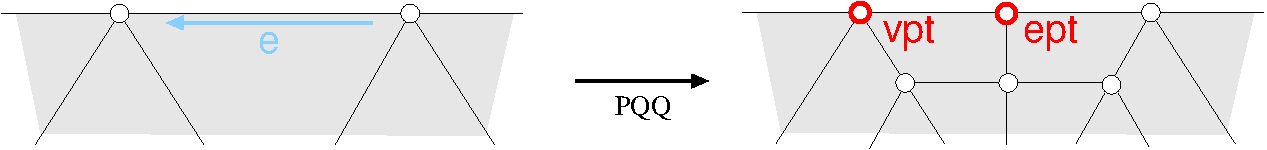
\includegraphics[width=0.75\textwidth]{Subdivision_method_3_ref/FIG/CCBorderMask}%
    }
  \end{center}
\end{ccTexOnly}

\begin{ccHtmlOnly}
    <CENTER>
      <img src="FIG/CCBorderMask.png" alt="PQQ stencil of border nodes"></A><P>
    </CENTER>
\end{ccHtmlOnly}

\ccHasModels

\ccRefIdfierPage{CGAL::CatmullClark_mask_3<Polyhedron_3>}

\ccSeeAlso

\ccRefIdfierPage{CGAL::Subdivision_method_3}

\end{ccRefConcept}

% +------------------------------------------------------------------------+
\ccRefPageEnd
% +------------------------------------------------------------------------+





% +------------------------------------------------------------------------+
\ccRefPageBegin
% +------------------------------------------------------------------------+

\begin{ccRefConcept}{PTQMask_3}
\label{pagePTQMaskRef}  

Required member functions for the \ccRefName\ concept. This
policy concept of geometric computations is used in
\ccc{CGAL::Subdivision_method_3::PTQ<Polyhedron_3, Mask>}.


%\ccTypes

%\ccNestedType{Point_3}{point type.}

\ccCreationVariable{mask}

\ccOperations
\ccSetThreeColumns{facet_node}{}{\hspace*{8.5cm}}

\ccMethod{void edge_node(Edge_handle e, Point_3& pt);}{
    computes the edge-point \ccc{pt} based on the neighborhood
    of the edge \ccc{e}.}

\ccMethod{void vertex_node(Vertex_handle v, Point_3& pt);}{
    computes the vertex-point \ccc{pt} based on the neighborhood
    of the vertex \ccc{v}.}

\ccMethod{void border_node(Halfedge_handle e, Point_3& ept, Point_3& vpt);}{
    computes the edge-point \ccc{ept} and the vertex-point \ccc{vpt} 
    based on the neighborhood of the border edge \ccc{e}.}

\begin{ccTexOnly}
  \begin{center}
    \parbox{0.75\textwidth}{%
      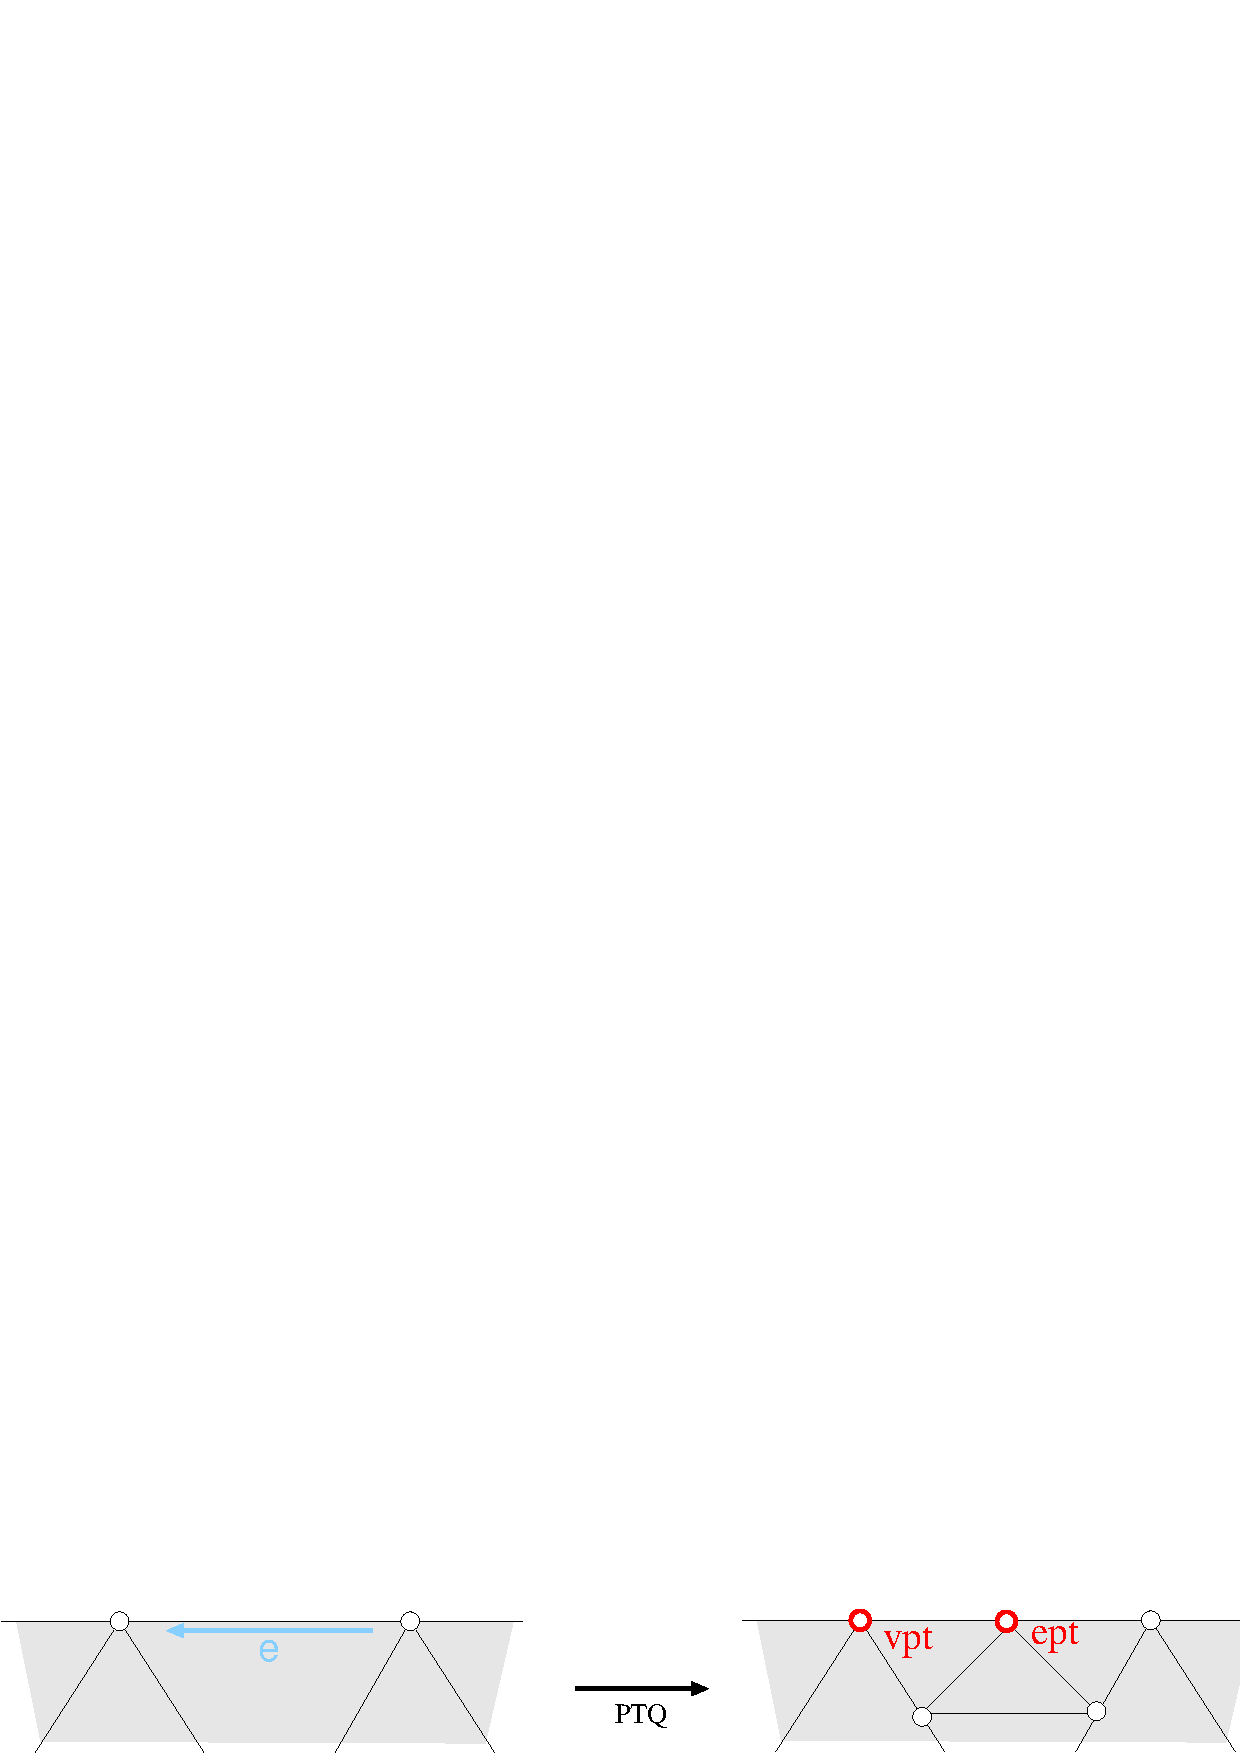
\includegraphics[width=0.75\textwidth]{Subdivision_method_3_ref/FIG/LoopBorderMask}%
    }
  \end{center}
\end{ccTexOnly}

\begin{ccHtmlOnly}
    <CENTER>
      <img src="FIG/LoopBorderMask.png" alt="PTQ stencil of border nodes"></A><P>
    </CENTER>
\end{ccHtmlOnly}

\ccHasModels

\ccRefIdfierPage{CGAL::Loop_mask_3<Polyhedron_3>}

\ccSeeAlso

\ccRefIdfierPage{CGAL::Subdivision_method_3}

\end{ccRefConcept}

% +------------------------------------------------------------------------+
\ccRefPageEnd
% +------------------------------------------------------------------------+






% +------------------------------------------------------------------------+
\ccRefPageBegin
% +------------------------------------------------------------------------+

\begin{ccRefConcept}{DQQMask_3}
\label{pageDQQMaskRef}  

Required member functions for the \ccRefName\ concept. This
policy concept of geometric computations is used in
\ccc{CGAL::Subdivision_method_3::DQQ<Polyhedron_3, Mask>}.


%\ccTypes

%\ccNestedType{Point_3}{point type.}

\ccCreationVariable{mask}

\ccOperations
\ccSetThreeColumns{facet_node}{}{\hspace*{8.5cm}}

\ccMethod{void corner_node(Halfedge_handle he, Point_3& pt);}{
    computes the subdivided point \ccc{pt} based on the neighborhood
    of the vertex pointed by the halfedge \ccc{he}.}

\begin{ccTexOnly}
  \begin{center}
    \parbox{0.55\textwidth}{%
      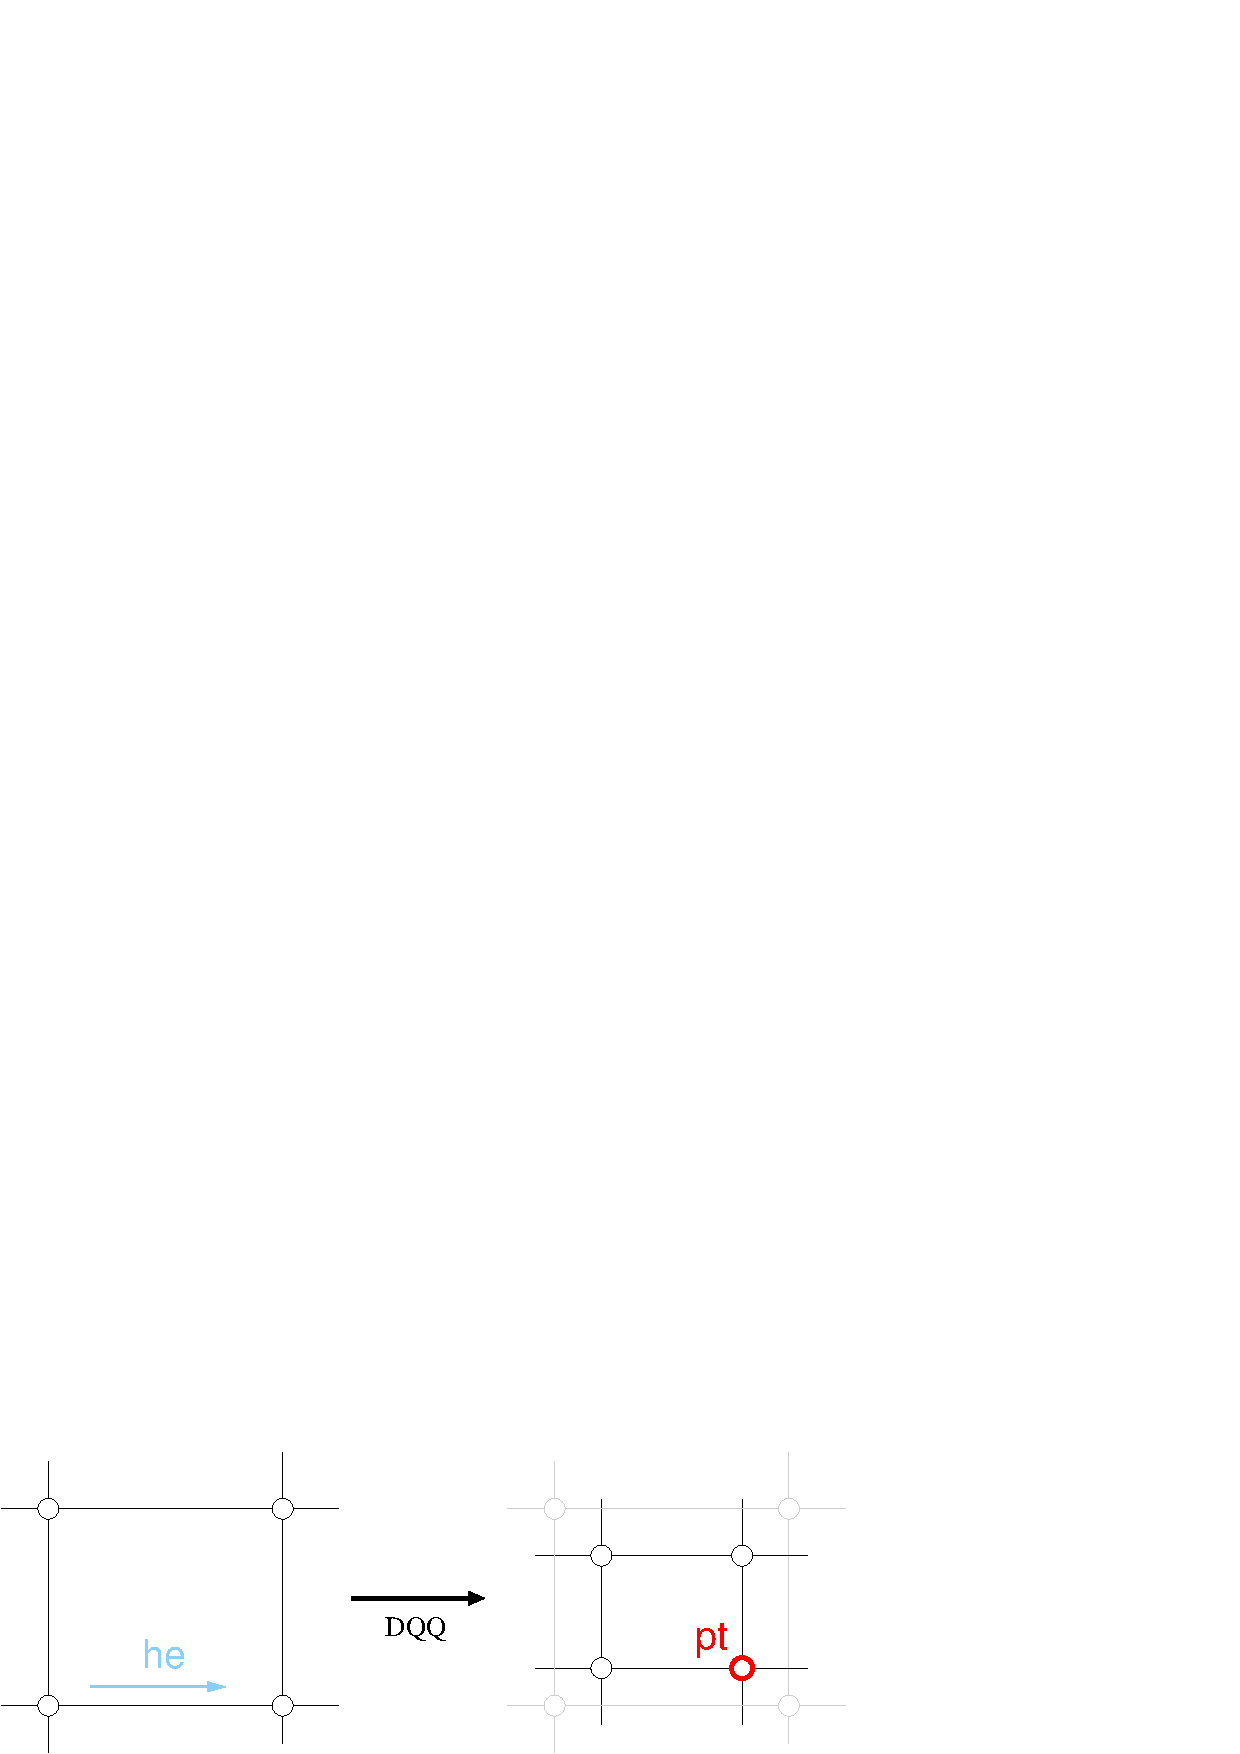
\includegraphics[width=0.55\textwidth]{Subdivision_method_3_ref/FIG/DSCornerMask}%
    }
  \end{center}
\end{ccTexOnly}

\begin{ccHtmlOnly}
    <CENTER>
      <img src="FIG/DSCornerMask.png" alt="DQQ corner stencil"></A><P>
    </CENTER>
\end{ccHtmlOnly}

\ccHasModels

\ccRefIdfierPage{CGAL::DooSabin_mask_3<Polyhedron_3>}

\ccSeeAlso

\ccRefIdfierPage{CGAL::Subdivision_method_3}

\end{ccRefConcept}

% +------------------------------------------------------------------------+
\ccRefPageEnd
% +------------------------------------------------------------------------+




% +------------------------------------------------------------------------+
\ccRefPageBegin
% +------------------------------------------------------------------------+

\begin{ccRefConcept}{Sqrt3Mask_3}
\label{pageSqrt3MaskRef}  

Required member functions for the \ccRefName\ concept. This
policy concept of geometric computations is used in
\ccc{CGAL::Subdivision_method_3::Sqrt3<Polyhedron_3, Mask>}.


%\ccTypes

%\ccNestedType{Point_3}{point type.}

\ccCreationVariable{mask}

\ccOperations
\ccSetThreeColumns{facet_node}{}{\hspace*{8.5cm}}

\ccMethod{void facet_node(Facet_handle f, Point_3& pt);}{
    computes the subdivided point \ccc{pt} based on the neighborhood
    of the facet \ccc{f}.}

\ccMethod{void vertex_node(Vertex_handle v, Point& pt);}{
    computes the subdivided point \ccc{pt} based on the neighborhood
    of the vertex \ccc{v}.}

\ccHasModels

\ccRefIdfierPage{CGAL::Sqrt3_mask_3<Polyhedron_3>}

\ccSeeAlso

\ccRefIdfierPage{CGAL::Subdivision_method_3}

\end{ccRefConcept}

% +------------------------------------------------------------------------+
\ccRefPageEnd
% +------------------------------------------------------------------------+
